
\documentclass[letterpaper,hide notes,xcolor={table,svgnames},pdftex,10pt]{beamer}
\def\showexamples{t}

\usecolortheme{crane}
\setbeamertemplate{navigation symbols}{}

\usetheme{MyPittsburgh}
\usepackage{hyperref}
\usepackage{graphicx,xspace}
\usepackage[normalem]{ulem}
\usepackage{multicol}
\usepackage{amsmath,amssymb,amsthm,graphicx,xspace}
\newcommand\SF[1]{$\bigstar$\footnote{SF: #1}}

\usepackage[sfdefault,lf]{carlito}
\usepackage[T1]{fontenc}
\usepackage[scaled]{beramono}
\usepackage{tikzpagenodes}
\newcommand{\Rplus}{\protect\hspace{-.1em}\protect\raisebox{.35ex}{\small{\small\textbf{+}}}}
\newcommand{\Cpp}{\mbox{C\Rplus\Rplus}\xspace}

\newcounter{tmpnumSlide}
\newcounter{tmpnumNote}

\newcommand\mnote[1]{%
	\addtocounter{tmpnumSlide}{1}
	\ifdefined\showcues {~\tiny\fbox{\arabic{tmpnumSlide}}}\fi
	\note{\setlength{\parskip}{1ex}\addtocounter{tmpnumNote}{1}\textbf{\Large \arabic{tmpnumNote}:} {#1\par}}}

\newcommand\mmnote[1]{\note{\setlength{\parskip}{1ex}#1\par}}


\newcommand\mquestion[2]{{~\color{red}\fbox{?}}\note{\setlength{\parskip}{1ex}\par{\Large \textbf{?}} #1} \note{\setlength{\parskip}{1ex}\par{\Large \textbf{A}} #2\par}\ifdefined \presentationonly \pause \fi}

\newcommand\blackboard[1]{%
	\ifdefined   \showblackboard
		{#1}
	\else {\begin{center} \fbox{\colorbox{blue!30}{%
						\begin{minipage}{.95\linewidth}%
							\hspace{\stretch{1}} Some space intentionally left blank; done at the blackboard.%
						\end{minipage}}}\end{center}}%
	\fi%
}

\usepackage{listings}
\lstset{%
	keywordstyle=\bfseries,
	aboveskip=15pt,
	belowskip=15pt,
	captionpos=b,
	identifierstyle=\ttfamily,
	frame=lines,
	numbers=left, basicstyle=\scriptsize, numberstyle=\tiny, stepnumber=0, numbersep=2pt}

\usepackage{siunitx}
\newcommand\sius[1]{\num[group-separator = {,}]{#1}\si{\micro\second}}
\newcommand\sims[1]{\num[group-separator = {,}]{#1}\si{\milli\second}}
\newcommand\sins[1]{\num[group-separator = {,}]{#1}\si{\nano\second}}
\sisetup{group-separator = {,}, group-digits = true}

%% -------------------- tikz --------------------
\usepackage{tikz}
\usetikzlibrary{positioning}
\usetikzlibrary{arrows,backgrounds,automata,decorations.shapes,decorations.pathmorphing,decorations.markings,decorations.text}

\tikzstyle{place}=[circle,draw=blue!50,fill=blue!20,thick, inner sep=0pt,minimum size=6mm]
\tikzstyle{transition}=[rectangle,draw=black!50,fill=black!20,thick, inner sep=0pt,minimum size=4mm]

\tikzstyle{block}=[rectangle,draw=black, thick, inner sep=5pt]
\tikzstyle{bullet}=[circle,draw=black, fill=black, thin, inner sep=2pt]

\tikzstyle{pre}=[<-,shorten <=1pt,>=stealth',semithick]
\tikzstyle{post}=[->,shorten >=1pt,>=stealth',semithick]
\tikzstyle{bi}=[<->,shorten >=1pt,shorten <=1pt, >=stealth',semithick]

\tikzstyle{mut}=[-,>=stealth',semithick]

\tikzstyle{treereset}=[dashed,->, shorten >=1pt,>=stealth',thin]

\usepackage{ifmtarg}
\usepackage{xifthen}
\makeatletter
% new counter to now which frame it is within the sequence
\newcounter{multiframecounter}
% initialize buffer for previously used frame title
\gdef\lastframetitle{\textit{undefined}}
% new environment for a multi-frame
\newenvironment{multiframe}[1][]{%
	\ifthenelse{\isempty{#1}}{%
		% if no frame title was set via optional parameter,
		% only increase sequence counter by 1
		\addtocounter{multiframecounter}{1}%
	}{%
		% new frame title has been provided, thus
		% reset sequence counter to 1 and buffer frame title for later use
		\setcounter{multiframecounter}{1}%
		\gdef\lastframetitle{#1}%
	}%
	% start conventional frame environment and
	% automatically set frame title followed by sequence counter
	\begin{frame}%
		\frametitle{\lastframetitle~{\normalfont(\arabic{multiframecounter})}}%
		}{%
	\end{frame}%
}
\makeatother

\makeatletter
\newdimen\tu@tmpa%
\newdimen\ydiffl%
\newdimen\xdiffl%
\newcommand\ydiff[2]{%
	\coordinate (tmpnamea) at (#1);%
	\coordinate (tmpnameb) at (#2);%
	\pgfextracty{\tu@tmpa}{\pgfpointanchor{tmpnamea}{center}}%
	\pgfextracty{\ydiffl}{\pgfpointanchor{tmpnameb}{center}}%
	\advance\ydiffl by -\tu@tmpa%
}
\newcommand\xdiff[2]{%
	\coordinate (tmpnamea) at (#1);%
	\coordinate (tmpnameb) at (#2);%
	\pgfextractx{\tu@tmpa}{\pgfpointanchor{tmpnamea}{center}}%
	\pgfextractx{\xdiffl}{\pgfpointanchor{tmpnameb}{center}}%
	\advance\xdiffl by -\tu@tmpa%
}
\makeatother
\newcommand{\copyrightbox}[3][r]{%
	\begin{tikzpicture}%
		\node[inner sep=0pt,minimum size=2em](ciimage){#2};
		\usefont{OT1}{phv}{n}{n}\fontsize{4}{4}\selectfont
		\ydiff{ciimage.south}{ciimage.north}
		\xdiff{ciimage.west}{ciimage.east}
		\ifthenelse{\equal{#1}{r}}{%
			\node[inner sep=0pt,right=1ex of ciimage.south east,anchor=north west,rotate=90]%
			{\raggedleft\color{black!50}\parbox{\the\ydiffl}{\raggedright{}#3}};%
		}{%
			\ifthenelse{\equal{#1}{l}}{%
				\node[inner sep=0pt,right=1ex of ciimage.south west,anchor=south west,rotate=90]%
				{\raggedleft\color{black!50}\parbox{\the\ydiffl}{\raggedright{}#3}};%
			}{%
				\node[inner sep=0pt,below=1ex of ciimage.south west,anchor=north west]%
				{\raggedleft\color{black!50}\parbox{\the\xdiffl}{\raggedright{}#3}};%
			}
		}
	\end{tikzpicture}
}


%% --------------------

%\usepackage[excludeor]{everyhook}
%\PushPreHook{par}{\setbox0=\lastbox\llap{MUH}}\box0}

%\vspace*{\stretch{1}

%\setbox0=\lastbox \llap{\textbullet\enskip}\box0}

\setlength{\parskip}{\fill}

\newcommand\noskips{\setlength{\parskip}{1ex}}
\newcommand\doskips{\setlength{\parskip}{\fill}}

\newcommand\xx{\par\vspace*{\stretch{1}}\par}
\newcommand\xxs{\par\vspace*{2ex}\par}
\newcommand\tuple[1]{\langle #1 \rangle}
\newcommand\code[1]{{\sf \footnotesize #1}}
\newcommand\ex[1]{\uline{Example:} \ifdefined \presentationonly \pause \fi
	\ifdefined\showexamples#1\xspace\else{\uline{\hspace*{2cm}}}\fi}

\newcommand\ceil[1]{\lceil #1 \rceil}


\AtBeginSection[]
{
	\begin{frame}
		\frametitle{Outline}
		\tableofcontents[currentsection]
	\end{frame}
}



\pgfdeclarelayer{edgelayer}
\pgfdeclarelayer{nodelayer}
\pgfsetlayers{edgelayer,nodelayer,main}

\tikzstyle{none}=[inner sep=0pt]
\tikzstyle{rn}=[circle,fill=Red,draw=Black,line width=0.8 pt]
\tikzstyle{gn}=[circle,fill=Lime,draw=Black,line width=0.8 pt]
\tikzstyle{yn}=[circle,fill=Yellow,draw=Black,line width=0.8 pt]
\tikzstyle{empty}=[circle,fill=White,draw=Black]
\tikzstyle{bw} = [rectangle, draw, fill=blue!20,
text width=4em, text centered, rounded corners, minimum height=2em]

\newcommand{\CcNote}[1]{% longname
	This work is licensed under the \textit{Creative Commons #1 3.0 License}.%
}
\newcommand{\CcImageBy}[1]{%
	\includegraphics[scale=#1]{creative_commons/cc_by_30.pdf}%
}
\newcommand{\CcImageSa}[1]{%
	\includegraphics[scale=#1]{creative_commons/cc_sa_30.pdf}%
}
\newcommand{\CcImageNc}[1]{%
	\includegraphics[scale=#1]{creative_commons/cc_nc_30.pdf}%
}
\newcommand{\CcGroupBySa}[2]{% zoom, gap
	\CcImageBy{#1}\hspace*{#2}\CcImageNc{#1}\hspace*{#2}\CcImageSa{#1}%
}
\newcommand{\CcLongnameByNcSa}{Attribution-NonCommercial-ShareAlike}

\newenvironment{changemargin}[1]{% 
	\begin{list}{}{% 
		\setlength{\topsep}{0pt}% 
		\setlength{\leftmargin}{#1}% 
		\setlength{\rightmargin}{1em}
		\setlength{\listparindent}{\parindent}% 
		\setlength{\itemindent}{\parindent}% 
		      \setlength{\parsep}{\parskip}% 
		      }% 
		\item[]}{\end{list}}




\title{Lecture 13 --- Semaphores }

\author{Jeff Zarnett \\ \small \texttt{jzarnett@uwaterloo.ca}}
\institute{Department of Electrical and Computer Engineering \\
  University of Waterloo}
\date{\today}


\begin{document}

\begin{frame}
  \titlepage

 \end{frame}

\begin{frame}
\frametitle{Mutual Exclusion through Messages}

The earlier definition of mutual exclusion was informal.

There are additional desirable properties that will be used to evaluate any solution:
\begin{itemize}
	\item Mutual exclusion must apply.
	\item A thread that halts outside the critical section must not interfere with other threads.
	\item It must not be possible for a thread requiring access to a critical section to be delayed indefinitely.
	\item When no thread is in the critical section, a thread that requests access should be allowed to enter right away.
	\item No assumptions are made about what the threads will do or the number of processors in the system.
	\item A thread remains inside the critical section for a finite time only.
\end{itemize}


\end{frame}

\begin{frame}
\frametitle{Back to Springfield}
Recall from earlier the example of the employees Alice and Bob who worked at the Springfield Nuclear Power Plant in Sector 7G.  

Suppose there is a third employee at the power plant, Charlie, who works on the day shift at the same time as Alice. 

Safety rules say that at least one of them has to monitor the safety of the reactor at all times and therefore they cannot both take lunch at the same time. 

If we cannot predict when lunch begins or how long it will last, how can Alice and Charlie co-ordinate to make sure they don't take lunch at the same time?

\end{frame}

\begin{frame}
\frametitle{At the Power Plant}

Before Alice gets up from her desk to go for lunch, she calls Charlie. 

If he does answer, she may proceed. 

If Charlie does not answer, Alice will know he is not at his desk.\\
\quad Therefore she cannot leave at the moment. 

She can call again, constantly, until she reaches Charlie (busy-waiting), but this ties up a phone line nonstop and is effort intensive for Alice. 

If she doesn't want to do that, at this point she has two options:\\
\quad Wait some period of time (perhaps 15 minutes) and call again. Or\\
\quad Leave a message in Charlie's voice mail box, asking him to call her back.

Then Alice can go about her work until she gets a call from Charlie and as soon as that happens, she may step out for lunch.


\end{frame}

\begin{frame}
\frametitle{Power Plant to Computer World}

Busy waiting has already been found inadequate as a solution. 

It wastes CPU time that another thread could be putting to productive use. 

The approach of ``wait 15 minutes and try again'' might be adequate for Alice as a human, but for the computer it is not ideal. 

If $A$ fails to get in, then sleeps for 2000~ms before trying again, if $B$ is finished after 20 ms, then thread $A$ waits unnecessarily for 1980~ms. 

What we want is something that resembles the call-when-finished semantics of Alice leaving a message and Charlie calling her back.

\end{frame}

\begin{frame}
\frametitle{Semaphore}

A semaphore is a system of signals used for communication. 

Before ships had radios, when two friendly ships were in visual range, they would communicate with one another through flag semaphores.

Each ship had someone holding certain flags in a specific position. 

Thus the two ships could co-ordinate at (visual range) distance.

This worked dramatically better than many alternatives (e.g., shouting).

\end{frame}

\begin{frame}
\frametitle{The Computer Semaphore}

The computer semaphore was invented in 1965 by Edsger Dijkstra.

He described a data structure that can be used to solve synchronization problems via messages. 

Although the version we use now is not exactly the same as the original description, even 50 years later, the core idea is unchanged.


\end{frame}

\begin{frame}
\frametitle{Binary Semaphore}

The \alert{binary semaphore}: this is a variable that has two values, 0 and 1. 

It can be initialized to 0 or to 1. 

The semaphore has two operations: \texttt{wait} and \texttt{signal}. 

In the original paper, \texttt{wait} was called \texttt{P} and \texttt{signal} was called \texttt{V}, but the names in common usage have become a little more descriptive. 

Note: \texttt{signal} is also called \texttt{post} in many textbooks.


\end{frame}

\begin{frame}
\frametitle{Binary Semaphore: wait}

The \texttt{wait} operation on the semaphore is how a program tries to enter the critical section.

 When \texttt{wait} is called, if the semaphore value is 1, set it to 0 and this thread may enter the critical section and continue. 
 
 If the semaphore is 0, some other thread is in the critical section and the current thread must \textit{wait} its turn. 
 
 The thread that called \texttt{wait} will be blocked by the operating system, just as if it asked for memory or a disk operation. 
 
 This is sometimes referred to as decrementing the semaphore (because the value changes from 1 to 0).

\end{frame}

\begin{frame}
\frametitle{Binary Semaphore: signal}

The \texttt{signal} operation is how a program \textit{signals}, or indicates, it is finished with the critical section. 

When this is called, if the semaphore is 1, do nothing.

If the semaphore is 0 and there is a task blocked awaiting that semaphore, that task may be unblocked.

Otherwise, set the semaphore to 1. 

This is also sometimes called incrementing the semaphore.

\end{frame}

\begin{frame}
\frametitle{Caffeine - the Stuff of Life?}

Analogy: you like coffee, and going to a particular coffee shop because there you can get your drink exactly the way you like it.

``Half caf, no whip, extra hot, extra foam, two shot, soy milk latte.''

After this beverage it may be the case that you need to use the washroom. 

The washroom is locked at such places, so to get in you will need the key, which is available by asking one of the employees. 

\end{frame}

\begin{frame}
\frametitle{Programmers Convert Caffeine into Code}

If nobody is currently in the washroom, you will get the key and can proceed. 

If it is currently occupied, you will have to wait. 

When the key is returned, if anyone is waiting, the employee will give the key to the first person in line for the washroom. 

Otherwise he or she will put the key away behind the counter.


\end{frame}

\begin{frame}
\frametitle{Semaphores: OS Support}

Observe that the operating system is needed to make this work. 

If thread $A$ attempts to wait on a semaphore that some other thread already has, it will be blocked. 

The operating system knows not to schedule it to run until it is unblocked. 

When thread $B$ is finished and signals the semaphore it is holding, that will unblock $A$ and allow it to run again.


\end{frame}

\begin{frame}
\frametitle{No Checking}


The semaphore does not provide any facility to ``check''the current value. 

A thread doesn't know in advance if it will block when it waits on a semaphore.

It can only give it a shot. Either it will be blocked or proceed directly.

\end{frame}

\begin{frame}
\frametitle{Signalling}

When a thread signals a semaphore, it likewise does not know if any other thread(s) are waiting on that semaphore. 

There is no facility to check this, either. 

When thread $A$ signals a semaphore, we don't know what thread will continue execution.


\end{frame}

\begin{frame}
\frametitle{Semaphore: Bad Behaviour}

Nothing in the semaphore as defined protects against certain bad behaviour.

Suppose thread $C$ would like to enter the critical section. 

The programmer of this task is malicious as well as impatient: ``my task is FAR too important to wait for those other processes and threads,'' he says. 

He implements his code: before he waits on the semaphore, he signals it. 

Even though $A$ or $B$ might be in the critical section, the semaphore is signalled.

So he is fairly certain that his program will now get to enter the critical section. 
\end{frame}

\begin{frame}
\frametitle{Semaphore: Bad Behaviour}

It's not foolproof: if there are other threads waiting, they might get woken up to proceed instead of $C$; much depends on the scheduler. 

Nevertheless, this is really bad: one process can wreak all kinds of havoc by letting another process into the critical section. 

Though the example here makes the author of thread $C$ a scheming villain, such a situation may occur if it is simply the result of a programming error.

\end{frame}

\begin{frame}
\frametitle{Preventing Bad Behaviour}

The problem identified is usually solved by supplementing the basic binary semaphore. 

A data structure called a \alert{mutex} is a binary semaphore with an additional rule enforced: only the thread that has called \texttt{wait} may \texttt{signal} that semaphore. 

This adds a small amount of extra bookkeeping to the semaphore, but this is a reasonable price to pay.

\end{frame}

\begin{frame}[fragile]
\frametitle{Semaphore Example: Linked List Integrity}

\begin{verbatim}
typedef struct single_node {
  void *element;
  struct single_node *next;
} single_node_t;

typedef struct single_list {
  single_node_t *head;
  single_node_t *tail;
  int size;
} single_list_t;


void single_list_init( single_list_t *list ) {
  list->head = NULL;
  list->tail = NULL;
  list->size = 0;
}
\end{verbatim}
\end{frame}

\begin{frame}[fragile]
\frametitle{Semaphore Example: Linked List Integrity}

\begin{verbatim}
bool push_front( single_list_t *list, void *obj ) {
  single_node_t *tmp = (single_node_t *) 
                  malloc( sizeof( single_node_t ) );
  
  if ( tmp == NULL ) {
    return false;
  }
  
  tmp->element = obj;
  tmp->next = list->head;
  list->head = tmp;

  if ( list->size == 0 ) {
     list->tail = tmp;
  }
  
   ++( list->size );
   return true;
}

\end{verbatim}
\end{frame}


\begin{frame}
\frametitle{Using the Linked List}

If only one thread access this data structure, we do not have a problem.

Suppose a thread tries to add an element $A$ to the list using \texttt{push\_front}. 

Right before the increment of the \texttt{size} fieldthere is a process switch. 

At this point, the new node has been allocated and initialized, the pointers of \texttt{head} and \texttt{tail} have been updated, but \texttt{size} is 0. 

\begin{center}
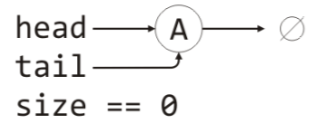
\includegraphics[width=0.25\textwidth]{images/linkedlist1.png}
\end{center}

\end{frame}

\begin{frame}
\frametitle{Using the Linked List}

Now, the second thread executes and wants to add $B$ to the linked list. 

In the conditional statement, \texttt{list->size == 0} evaluates to true. 

Thus, the \texttt{tail} pointer is updated.

\begin{center}
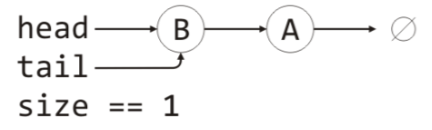
\includegraphics[width=0.35\textwidth]{images/linkedlist2.png}
\end{center}


\end{frame}

\begin{frame}
\frametitle{Using the Linked List}

When the first thread gets to run again, it will resume where it left off. 

It increments the \texttt{size} integer, leaving the final state: \texttt{head} and \texttt{tail} both point to element $B$, even though there is element $A$ in the list.

\begin{center}
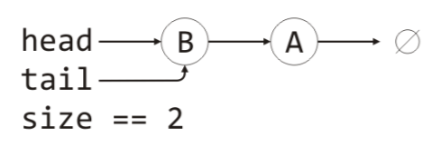
\includegraphics[width=0.35\textwidth]{images/linkedlist3.png}
\end{center}


\end{frame}

\begin{frame}
\frametitle{Inconsistent State}

This is an \alert{inconsistent state}.

The linked list has two elements in it but the \texttt{tail} pointer is wrong. 

An attempt to remove an element from the list will reveal the problem.

Remove the front element? Check if \texttt{head} and \texttt{tail} are equal. That may give the mistaken impression that $B$ is the last element in the list. We lost $A$!

Or the \texttt{head} pointer will be updated but \texttt{tail} will still point to $B$ even after it has been freed, which can result in a segmentation fault or invalid access.


\end{frame}

\begin{frame}
\frametitle{Binary Semaphore Syntax}

The linked list problem just discussed can be solved easily if a semaphore is employed. 

The syntax we will use is as follows:

\texttt{semaphore\_init( semaphore\_t *sem, int i )}\\
Initialize the semaphore to \texttt{i} (can be 0 or 1).

\texttt{semaphore\_wait( semaphore\_t *sem )}\\
Wait on a semaphore.

\texttt{semaphore\_signal( semaphore\_t *sem)}\\
If the semaphore is 1, do nothing.\\
If the semaphore is 0 and there is at least one task blocked on this semaphore, unblock it; otherwise set the semaphore to 1.

\end{frame}

\begin{frame}[fragile]
\frametitle{Applying the Semaphore to the Linked List}

\begin{verbatim}
typedef struct single_node {
  void *element;
  struct single_node *next;
} single_node_t;

typedef struct single_list {
  single_node_t *head;
  single_node_t *tail;
  int size;
  semaphore_t mutex;
} single_list_t;

void single_list_init( single_list_t *list ) {
  list->head = NULL;
  list->tail = NULL;
  list->size = 0;

  semaphore_init( &( list->mutex ), 1 );
}
\end{verbatim}

\end{frame}

\begin{frame}[fragile]
\frametitle{Applying the Semaphore to the Linked List}

\begin{verbatim}
bool push_front( single_list_t *list, void *obj ) {
  single_node_t *tmp = (single_node_t *) 
                   malloc( sizeof( single_node_t ) );
  
  if ( tmp == NULL ) { return false; }  
  tmp->element = obj;

  semaphore_wait( &( list->mutex ) ); {  
    tmp->next = list->head;
    list->head = tmp;

    if ( list->size == 0 ) {
       list->tail = tmp;
    }
    ++( list->size );
  
  } semaphore_signal( &( list->mutex ) );
  return true;
}
\end{verbatim}


\end{frame}

\begin{frame}
\frametitle{Applying the Semaphore to the Linked List}

The critical section here just encloses the modification of the shared linked list. 

In theory one might put the wait and signal operations at the start and end of the entire function, respectively. 

This is, however, suboptimal: it forces unnecessary waiting. 

Including the call to \texttt{malloc} is especially bad; the memory allocation itself can block if insufficient memory is available. 

\end{frame}

\begin{frame}
\frametitle{Counting Semaphores}

Binary semaphores are useful, and we can generalize this concept to what is known as a \alert{counting} or \alert{general} semaphore. 

Instead of having only the values 0 and 1, the setup routine for the counting semaphore allows the choice of an integer value and this is the maximum value. 

A thread that waits on that semaphore will decrement the integer by 1.

A thread that signals on the semaphore will increment the integer by 1. 

\end{frame}


\begin{frame}
\frametitle{General Semaphores}

If a thread attempts to wait on a semaphore and the decrement operation makes the integer value negative, the calling thread is blocked. 

If initialized with 5 and the current value is 2, a thread that waits on that general semaphore will not be blocked.

In some operating systems there is no distinction between binary and counting semaphores (create a general semaphore with a value of 1).

\end{frame}


\begin{frame}
\frametitle{General Semaphore Creation}

The general semaphore initialization function signature now takes an extra parameter, \texttt{n}, to show the maximum value of the semaphore.

\texttt{semaphore\_init( semaphore\_t *sem, int i, int n )}\\
Initialize the semaphore to \texttt{i} with a maximum value of \texttt{n}.


\end{frame}


\end{document}

